\chapter{其他约化群的Langlands对应III：对应的表述}\label{L20}\lecturedate{2020/04/27}\sourcepage{165}
设$F$为非阿基米德局部域，$\OO_F$为其整数环。% [Tutor Note: 原书 p165 作「Let $F$ be a local field」（未排除阿基米德情形）；本讲只用到非阿基米德情形，译文按此收紧。]设$G$为$F$上的分裂约化群，并选取其分裂约化$\OO_F$模型和在$\OO_F$上定义的极大分裂环面$T$。以$X,X^\vee$分别表示$T$的代数特征标格和余特征标格。\lref{L19}介绍了Satake同构
\begin{equation}\tag{0.1}\label{L20eq01}\mathcal H=\mathcal H(G(F),G(\OO_F))\cong\C[X^\vee]^W.\end{equation}
这一同构把每个$f\in\mathcal H$送到它的Fourier变换$\widehat f$。

以$G^L$表示$G$的Langlands对偶群，$T^L$为其中的极大环面。于是$X,X^\vee$分别是$T^L$的余特征标格和特征标格。由\eref{定理}{L18S2O7}，$G^L(\C)$的不可约有理表示与其支配权一一对应。另一方面，$G^L(\C)$约化，因而线性约化，每个有限维有理表示都是不可约表示的直和。
\section{\texorpdfstring{$\C[X^\vee]^W$}{C[X∨]的W不变环}的两组基}\label{L20S1}\idx{Weyl特征标}\idx{表示环}
由\eqref{L20eq01}中的Satake同构，$\{\widehat c_\lambda\}_{\lambda\in(X^\vee)^+}$给出$\C[X^\vee]^W$的一组基。

另一方面，对应于支配权$\lambda$的$G^L(\C)$的不可约表示$V_\lambda$，其\textbf{Weyl特征标}定义为
\begin{equation}\tag{1.1}\label{L20eq11}
\operatorname{Ch}(V_\lambda):=\sum_{\gamma\in X^\vee}\dim V_\lambda(\gamma)e^\gamma
=\frac{\sum_{w\in W}(-1)^{\ell(w)}e^{w(\lambda+\kappa^\vee)-\kappa^\vee}}{\prod_{\alpha^\vee\in\Phi^\vee_+}(1-e^{-\alpha^\vee})}.
\end{equation}
% [Tutor Note: 原书 p165 的 (1.1) 分母作 $\sum_{\alpha^\vee\in\Phi^\vee_+}(1-e^{-\alpha^\vee})$（求和号），应为乘积 $\prod$；译文按正确写法处理。]
\sourcepage{166}
这里，作为$T^L(\C)$模，$V_\lambda$具有权空间分解$V_\lambda=\bigoplus_{\gamma\in X^\vee}V_\lambda(\gamma)$，而$\kappa^\vee=\frac12\sum_{\alpha^\vee\in\Phi^\vee_+}\alpha^\vee$。容易看出，$\operatorname{Ch}(V_\lambda)$为$W$不变量，并构成$\C[X^\vee]^W$的一组基。还可为任意有限维有理表示定义Weyl特征标，使
\[\operatorname{Ch}(V_1\oplus V_2)=\operatorname{Ch}(V_1)+\operatorname{Ch}(V_2).\]
因此映射$V\mapsto\operatorname{Ch}(V)\in\C[X^\vee]^W$给出复化表示环$\operatorname{Rep}G^L(\C)\otimes_{\Z}\C$与$\C[X^\vee]^W$的同构。

现在，$\C[X^\vee]^W$有两组基$\{\widehat c_\lambda\}_{\lambda\in(X^\vee)^+}$和$\{\operatorname{Ch}(V_\lambda)\}_{\lambda\in(X^\vee)^+}$。写成
\begin{equation}\tag{1.2}\label{L20eq12}\operatorname{Ch}(V_\lambda)=\sum_{\gamma\in(X^\vee)^+}d_{\lambda\gamma}\widehat c_\gamma.\end{equation}
\originalnumber{1}
\begin{lemma}\label{L20S1O1}设$d_{\lambda\gamma}$如\eqref{L20eq12}。除非$\gamma\le\lambda$，否则$d_{\lambda\gamma}=0$。\end{lemma}
\begin{proof}
由\lref{L19}末给出的公式，
\begin{align*}
\widehat c_\gamma&=\sum_{\nu\in X^\vee}\widetilde c_\gamma(\pi^\nu)e^\nu
=\sum_{\nu\in(X^\vee)^+}\widetilde c_\gamma(\pi^\nu)\left(\sum_{w\in W/W_\nu}e^{w(\nu)}\right)\\
&=\sum_{\nu\in(X^\vee)^+}\delta(\pi^\nu)^{1/2}\int_{U(F)}c_\gamma(\pi^\nu u)\,d\mu_U(u)\left(\sum_{w\in W/W_\nu}e^{w(\nu)}\right),
\end{align*}
% [Tutor Note: 原书 p166 的 (1.2) 证明中作 $e^{-\nu}$、$e^{-w(\nu)}$，译文用 $e^{\nu}$、$e^{w(\nu)}$，与上一讲 $c_\lambda\mapsto e^\lambda$ 的约定一致。]
其中$\delta$为$T(F)$上的模特征标，$W_\nu$为$\nu$在$W$中的稳定子群，$U(F)$为所选正根对应的$G$的Borel子群$B$的幂幺根基，$\mu_U$为$U(F)$上的Haar测度，归一化为$\mu_U(U(\OO_F))=1$。按定义，
% [Tutor Note: 原书 p166 称 $U(F)$ 为「与 $G^L$ 的正根选取相对应的 Borel 子群的幂幺根基」，此处应为 $G$ 的正根（$\delta$ 由 $G$ 的根空间计算）；译文按正确写法处理。]
\[\widetilde c_\gamma(\pi^\nu)=\delta(\pi^\nu)^{1/2}\mu_U\bigl(\pi^{-\nu}G(\OO_F)\pi^\gamma G(\OO_F)\cap U(F)\bigr).\]
由下面的\eref{引理}{L20S1O2}，除非$\nu\le\gamma$，否则$\widetilde c_\gamma(\pi^\nu)=0$。因此，只有有限多个$\nu\in(X^\vee)^+$使$\widetilde c_\gamma(\pi^\nu)\ne0$。

此外，$\widetilde c_\gamma(\pi^\gamma)\ne0$，因为
\[\pi^\gamma U(F)\cap G(\OO_F)\pi^\gamma G(\OO_F)\supseteq\pi^\gamma\bigl(U(F)\cap G(\OO_F)\bigr),\]
且$\mu_U(U(F)\cap G(\OO_F))=\mu_U(U(\OO_F))=1$。

另一方面，对支配权$\nu$，只有$\nu\le\lambda$时，$\dim V_\lambda(\nu)$才可能非零。由两组基的三角形展开及\eqref{L20eq12}右端的有限性，得到：对任何不满足$\gamma\le\lambda$的$\gamma$，都有$d_{\lambda\gamma}=0$。
\end{proof}
\originalnumber{2}
\begin{lemma}\label{L20S1O2}
若$\pi^\nu U(F)\cap G(\OO_F)\pi^\gamma G(\OO_F)\ne\varnothing$，其中$\nu\in X^\vee$、$\gamma\in(X^\vee)^+$，则$\nu\le\gamma$。
\end{lemma}
\sourcepage{167}
\eref{引理}{L20S1O2}的证明见\bref{L20S}{S}第7.2、7.3节。

按定义，$\delta(\pi^\nu)^{1/2}=q^{-\langle\kappa,\nu\rangle}$，其中$\kappa=\frac12\sum_{\alpha\in\Phi_+}\alpha$，$q=|\OO_F/\mathfrak m|$。对$\gamma\in(X^\vee)^+$，定义
\[a^\nu_\gamma:=\mu_U\bigl(\pi^{-\nu}G(\OO_F)\pi^\gamma G(\OO_F)\cap U(F)\bigr).\]
若$g$属于这一交集，则整个右陪集$gU(\OO_F)$也属于交集。因此$a^\nu_\gamma$是非负整数；它或者为零，或者至少为$1$。对任意$w\in W$，还有
\[q^{-\langle\kappa,\nu\rangle}a^\nu_\gamma=q^{-\langle\kappa,w(\nu)\rangle}a^{w(\nu)}_\gamma,\]
以及
\begin{equation}\tag{1.3}\label{L20eq13}\widehat c_\gamma=\sum_{\nu\in X^\vee}q^{-\langle\kappa,\nu\rangle}a^\nu_\gamma e^\nu.\end{equation}
% [Tutor Note: 原书 p167 的 (1.3) 作 $e^{-\nu}$，译文用 $e^{\nu}$，同上一条的符号约定。]
有以下Lusztig的定理，见\bref{L20L}{L}。
\originalnumber{3}
\begin{theorem}\label{L20S1O3}
设$d_{\lambda\gamma}$如\eqref{L20eq12}，则$p_{\lambda\gamma}:=q^{\langle\kappa,\lambda\rangle}d_{\lambda\gamma}$为$q$的多项式，并且$p_{\lambda\gamma}(1)=\dim V_\lambda(\gamma)$。
\end{theorem}
有
\begin{equation}\tag{1.4}\label{L20eq14}\sum_{\gamma\in(X^\vee)^+}p_{\lambda\gamma}a^\nu_\gamma=q^{\langle\kappa,\lambda+\nu\rangle}\dim V_\lambda(\nu).\end{equation}
由于不满足$\gamma\le\lambda$时$p_{\lambda\gamma}=0$，而只要存在$w\in W$使$w(\nu)\not\le\gamma$，就有$a^\nu_\gamma=0$，所以$p_{\lambda\gamma}a^\nu_\gamma\ne0$仅可能发生在对所有$w\in W$均有$w(\nu)\le\gamma\le\lambda$的情形。令$w_0$为Weyl群的最长元，取$\nu=w_0\lambda$，得到
\[p_{\lambda\lambda}a^{w_0\lambda}_\lambda=\dim V_\lambda(w_0\lambda)=1=p_{\lambda\lambda}(1).\]
% [Tutor Note: 原书 p167 取 ν=−λ，本处取 ν=w_0λ；两者由 w_0 置换对应，结论一致。]
由于$a^{w_0\lambda}_\lambda\ge1$，有
\[\begin{cases}p_{\lambda\lambda}=\dim V_\lambda(\lambda)=p_{\lambda\lambda}(1)=1,\\a^{w_0\lambda}_\lambda=1.\end{cases}\]
于是矩阵$(p_{\lambda\gamma})$为单位上三角矩阵，\eqref{L20eq14}中的线性方程的解可表示为$q$的多项式。因此证明了以下推论。
\originalnumber{4}
\begin{corollary}\label{L20S1O4}$a^\nu_\gamma$为$q$的多项式。\end{corollary}
回忆，$\mathcal H$的结构常数定义为
\[c_\lambda*c_\gamma=\sum_{\beta\in(X^\vee)^+}c^\beta_{\lambda\gamma}c_\beta,\qquad\lambda,\gamma\in(X^\vee)^+.\]
\sourcepage{168}
\originalnumber{5}
\begin{corollary}\label{L20S1O5}$c^\beta_{\lambda\gamma}$为$q$的多项式。\end{corollary}
\begin{proof}
\eqref{L20eq01}中的Satake同构为代数同态，所以
\[\sum_{\beta\in(X^\vee)^+}c^\beta_{\lambda\gamma}\widehat c_\beta=\widehat{c_\lambda*c_\gamma}=\widehat c_\lambda\,\widehat c_\gamma.\]
因此
\[\sum_{\beta\in(X^\vee)^+}c^\beta_{\lambda\gamma}q^{-\langle\kappa,\nu\rangle}a^\nu_\beta=\sum_{\nu_1+\nu_2=\nu}q^{-\langle\kappa,\nu\rangle}a^{\nu_1}_\lambda a^{\nu_2}_\gamma,\]
从而
\[\sum_{\beta\in(X^\vee)^+}c^\beta_{\lambda\gamma}a^\nu_\beta=\sum_{\nu_1+\nu_2=\nu}a^{\nu_1}_\lambda a^{\nu_2}_\gamma.\]
由\eref{推论}{L20S1O4}，右端为$q$的多项式。取$\nu=w_0\eta$时，矩阵$(a^{w_0\eta}_\beta)$也是单位上三角的，因此逐项求解可知$c^\beta_{\lambda\gamma}$为$q$的多项式。
\end{proof}

\section{Langlands函子性}\label{L20S2}\idx{Langlands函子性}\idx{L群}
上一讲定义的带状球函数，见\eref{定义}{L19S3O3}，正是归一化的Hecke特征函数。% [Tutor Note: 原书 p168 引作「Definition 3.4 in Lecture 19」，实为定义 3.3（该讲顺序为定理 3.1、注记 3.2、定义 3.3）；译文引用正确。]
由\eref{定理}{L19S3O5}，这些特征函数与
\[(X\otimes\C)\big/\bigl(W\ltimes(2\pi iX')\bigr),\qquad X'=\{s\in X\otimes\C\mid\langle s,\lambda\rangle\in\Z,\ \lambda\in X^\vee\},\]
中的元素一一对应。
\originalnumber{1}
\begin{note}[L20S2O1]
上述商空间可看作$G^L(\C)$的半单共轭类集合。选取$X$的一组基$x_1,\ldots,x_r$，把$s=\sum b_jx_j\in X\otimes\C$对应到$G^L(\C)$中的元素$\prod_jx_j(e^{-b_j})$。注意，$x_j\in X$可视为对偶环面$T^L$的一参数余特征标。该对应诱导上述商空间与$G^L(\C)$半单共轭类集合之间的同构。
\end{note}
% [Tutor Note: 原书 p168 的注记 2.1 作 $\prod_j x_j(e^{b_j})$（译文用 $e^{-b_j}$，符号约定同上），并称 $x_i\in X$「可视为 $T$ 的一参数子环面」，此处应为对偶环面 $T^L$ 的一参数子群；译文按正确写法处理。]
每个Hecke特征函数$\omega$给出同态$\mathcal H\to\C$，$f\mapsto\widehat\omega(f)$。此外，有以下交换图：
\begin{figure}[H]\centering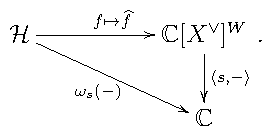
\includegraphics[width=0.2192\paperwidth]{images/L20-p168-Satake.pdf}\end{figure}
\sourcepage{169}
综合上述结果，有以下定理。
\originalnumber{2}
\begin{theorem}\label{L20S2O2}
球面Hecke代数$\mathcal H(G(F),G(\OO_F))$同构于$\operatorname{Rep}G^L(\C)\otimes_{\Z}\C$，其中$G^L(\C)$为$G$的Langlands对偶群。$\C$代数同态$\mathcal H(G(F),G(\OO_F))\to\C$的集合与$G^L(\C)$的半单共轭类集合之间存在双射。
\end{theorem}
\eref{定理}{L20S2O2}可看作非阿基米德局部域上非分歧情形的局部Langlands对应\znote{局部 Langlands 对应猜想：$G(F)$ 的不可约光滑表示应与 $L$ 参数（$W_F\times\SL_2$ 到 $G^L$ 的连续同态类）一一对应，并使两边的 $L$ 函数与 $\varepsilon$ 因子相符。未分歧情形即本讲定理 2.2：表示由半单共轭类（Satake 参数）决定，而对任意分裂约化群这一情形已经成立。$\GL_n$ 的一般情形是已知定理。它是整体 Langlands 对应的局部构件。[来源：S. Gelbart, \textit{An elementary introduction to the Langlands program}, Bull. Amer. Math. Soc. 10 (1984) 177--219（本讲参考文献 [G]）。]}。之所以称为非分歧情形，是因为定义带状球函数的拟特征标在$T(\OO_F)$上的限制为平凡特征标。关于局部Langlands猜想，还有其他结果，见\bref{L20BG}{BG}。

但在整体情形，对应关系无法像$\GL_n$情形那样清晰地一一配对。我们将简要介绍\textbf{Langlands函子性}\znote{Langlands 函子性说：每个 $L$ 同态 $f:G^L\to G'^L$ 都应诱导自守表示的转移，把 $G$ 的自守表示送到 $G'$ 的自守表示，并使两边的 $L$ 函数一致。它把 Langlands 猜想统一到约化群：取 $G'=\GL_n$ 可把一般 $G$ 的 $L$ 函数归约到 $\GL_n$ 的已知理论，取 $G$ 平凡则回到互反猜想。已证情形包括内形之间的 Jacquet--Langlands 对应、经典群的内窥理论，以及对称幂函子性的部分情形。[来源：nLab "Langlands functoriality"，\url{https://ncatlab.org/nlab/show/Langlands+functoriality}（Last revised 2022-11-23；2026-11-14 访问）。]}，它最终把Langlands猜想推广到约化群。也可参看\bref{L20BG}{BG}或\bref{L20G}{G}。

设$\A_F$为整体域$F$的阿代尔环。先回顾对$G=\GL_n$已经讨论的结果。
\begin{enumerate}[label=\arabic*.]
\item \textbf{从局部到整体。}每个$G(\A_F)$的不可约可容许表示都可写为局部不可约可容许表示$\rho_v$的限制张量积$\bigotimes'_v\rho_v$。限制张量积相对于一族向量$(u_v^0)$定义，对几乎所有有限地方$v$，有$u_v^0\in\rho_v^{G(\OO_v)}$。
\item 整体Hecke代数由局部Hecke代数的限制张量积定义：
\[\mathcal H(G(\A_F),K):=\bigotimes'_v\mathcal H(G(F_v),\GL_n(\OO_v)).\]
整体Hecke代数作用于尖点自守形式空间$\mathcal A_0(G)$。\znoteplain{原书写 $\bigotimes'_v$ 表示对全部地方取限制张量积；在数域情形，几乎所有的局部因子都由 $\GL_n(\OO_v)$ 的球面 Hecke 代数给出，而 $v$ 有限时 $\mathcal H(G(F_v),\GL_n(\OO_v))$ 正是球面 Hecke 代数，故整体代数可拆成「有限部分 $K_f$」与「无穷处的相应代数」两部分，二者在尖点形式空间上的作用可以分开处理。（上下文推断，无外部依据）}
\item \textbf{重数一。}$G(\A_F)$的不可约表示在$\mathcal A_0(G)$中的重数不超过$1$。
\item \textbf{强重数一。}若$\rho_1,\rho_2\subseteq\mathcal A_0(G)$，且几乎所有$v$处的$\rho_{1,v},\rho_{2,v}$同构，则作为$\mathcal A_0(G)$的子空间，$\rho_1=\rho_2$。
\sourcepage{170}
\item Chebotarev密度定理保证，在半单化意义下，除有限多个地方以外的所有Frobenius共轭类唯一确定$\GL_n$值Galois表示。
\item 不可约自守表示与在自守空间中出现的不可约Hecke模相对应。几乎所有地方的球面Hecke特征函数给出$G^L$中的共轭类；在Langlands对应下，这些类与Galois表示给出的Frobenius共轭类逐处对应。换言之，有下图中的对应关系。
\end{enumerate}
\begin{figure}[H]\centering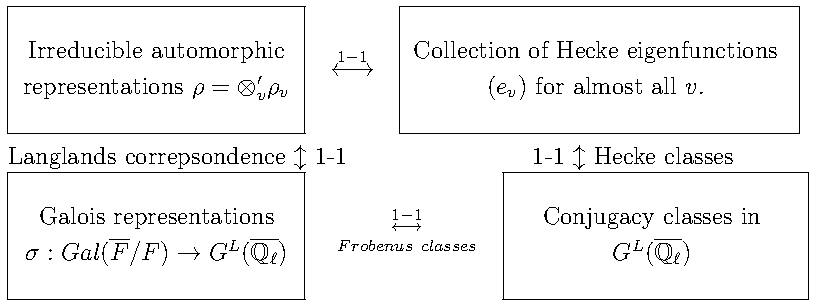
\includegraphics[width=0.6576\paperwidth]{images/L20-p170-correspondence.pdf}\end{figure}
一般连通约化群$G$不具备上述第3、4条性质，第5条所述的唯一性也不能直接推广为任意$G^L$值表示的唯一性。因此，不能为一般约化群照搬第6条所描述的猜想。

虽然无法普遍建立表示之间简单的一一对应，我们仍可在数值层面提出猜想，即通过$L$函数来表述。事实上，$\GL_n$的Langlands猜想可用$L$函数\znote{$L$ 函数把局部数据（$t(\rho_v)$ 与 $\sigma(\operatorname{Fr}[v])$）乘成整体 Euler 乘积，Langlands 猜想的核心正是这些乘积的解析延拓与函数方程：自守侧与 Galois 侧的非分歧 Euler 因子逐处相同，从而两个 $L$ 函数相等。乘积中的 $S$ 必须包含全部分歧地方与无穷地方，否则因子未必收敛；对 $\GL_n$，自守 $L$ 函数的解析性质可由积分表示得到，而 Artin $L$ 函数一侧则来自 Galois 表示。[来源：S. Gelbart, \textit{An elementary introduction to the Langlands program}, Bull. Amer. Math. Soc. 10 (1984) 177--219（本讲参考文献 [G]）。]}重述为下列猜想。
\originalnumber{3}
\begin{conjecture}[Langlands互反猜想]\label{L20S2O3}
设$L/k$为整体域的有限Galois扩张，其Galois群为$\Gal(L/k)$，$\sigma:\Gal(L/k)\to\GL_n(\C)$为不可约表示。则存在$k$上的尖点自守表示$\rho_\sigma$，使
\[L(s,\rho_\sigma)=L(s,\sigma).\]
\end{conjecture}
上述两个$L$函数在非分歧有限地方的Euler因子为
\[L^S(s,\rho)=\prod_{v\notin S}\det\bigl(I-t(\rho_v)q_v^{-s}\bigr)^{-1},\qquad L^S(s,\sigma)=\prod_{v\notin S}\det\bigl(I-\sigma(\operatorname{Fr}[v])q_v^{-s}\bigr)^{-1},\]
其中$S$包含分歧地方及无穷地方。
\sourcepage{171}
这里$t(\rho_v)$为$\rho_v$在$\GL_n(\C)$中的半单共轭类，$q_v$为$v$处剩余域的元素个数。

设$G$为在域$k$上定义的任意连通约化群，$L/k$为充分大的有限Galois扩张，使其上$G$分裂。可定义复约化群$G^L_0$及$\Gal(L/k)$在其上的作用。半直积
\[G^L:=G^L_0\rtimes\Gal(L/k)\]
具有以下性质。
\begin{enumerate}[label=\arabic*.]
\item 若$G$在$k$上分裂，则$G^L_0$为其Langlands对偶群，$G^L$为直积，即$\Gal(L/k)$在$G^L_0$上的作用平凡。
\item 一般而言，若$v$在$L$中非分歧，且$G$在$v$处为非分歧群，选取一个对应的Frobenius元素$\operatorname{Fr}[v]$，则$G(k_v)$的不可约非分歧表示\znote{设 $G$ 在 $F$ 上分裂。$G(F)$ 的不可约光滑表示称为\textbf{未分歧}的，若它有非零的 $G(\OO_F)$-不变向量；此时不变向量空间是一维，表示由它在球面 Hecke 代数上的特征（即 Satake 参数）唯一确定。对 $\GL_n$，未分歧性在 Galois 侧表现为 $\sigma$ 在 $v$ 处未分歧，而 Satake 参数正是 $\sigma(\operatorname{Fr}_v)$ 的半单共轭类，这就是上文第 6 条所说的逐处对应。[来源：J. Bernstein, S. Gelbart (eds.), \textit{An introduction to the Langlands Program}, Birkhäuser 2004, 第 11 章（J. W. Cogdell）（本讲参考文献 [BG]）。]}$\rho_v$与相应的半单Satake参数$t(\rho_v)\in G^L$的$G^L_0$共轭类一一对应，其在$\Gal(L/k)$中的投影为$\operatorname{Fr}[v]$。
\end{enumerate}
$G^L$称为$G$的\textbf{$L$群的Galois形式}\znote{$L$ 群把对偶群与 Galois 作用打包在一起：$G^L=G^L_0\rtimes\Gal(L/k)$。$G$ 分裂时作用平凡，$G^L$ 退化为对偶群；一般情形下，$G(k_v)$ 的未分歧表示对应 $G^L$ 中的共轭类 $t(\rho_v)$，它在 $\Gal(L/k)$ 上的投影必须是 $\operatorname{Fr}[v]$，于是分歧的形状被记录进 $L$ 群的结构。$L$ 同态是与之相容的连续同态，且在 $G^L_0$ 上的限制为代数同态。[来源：J. Bernstein, S. Gelbart (eds.), \textit{An introduction to the Langlands Program}, Birkhäuser 2004, 第 11 章（J. W. Cogdell）（本讲参考文献 [BG]）。]}。$G^L$的表示是同态$r:G^L\to\GL_n(\C)$，要求其在$G^L_0$上的限制为复解析的。两个$L$群$G^L,G'^L$之间的\textbf{$L$同态}是连续同态$h:G^L\to G'^L$，在连通对偶群上的限制为代数同态，并与两群到$\Gal(L/k)$的自然投影相容，如下交换图所示。
\begin{figure}[H]\centering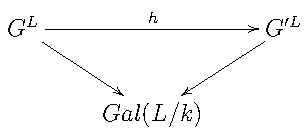
\includegraphics[width=0.2485\paperwidth]{images/L20-p171-Lhom.pdf}\end{figure}
% [Tutor Note: 原书 p171 未写此条，此处按 $L$ 同态的标准定义补足，不改变命题内容。]
于是有以下两个猜想。
\originalnumber{4}
\begin{conjecture}\label{L20S2O4}
设$\rho=\bigotimes'_v\rho_v$为$G$的自守表示，$r$为$G^L$的有限维表示。有Euler乘积
\begin{equation}\tag{2.1}\label{L20eq21}L^S(s,\rho,r)=\prod_{v\notin S}\det\bigl(I-r(t(\rho_v))q_v^{-s}\bigr)^{-1},\end{equation}
其中$S$包括全部分歧地方和无穷地方。这一最初在$s$的某个右半平面定义的$L$函数，可亚纯延拓到整个$\C$，并有联系$L^S(s,\rho,r)$与$L^S(1-s,\widetilde\rho,r)$的函数方程，其中$\widetilde\rho$为逆表示。
\end{conjecture}
\sourcepage{172}
\originalnumber{5}
\begin{conjecture}[关于$L$群的自守形式函子性]\label{L20S2O5}
设$G,G'$为约化群，$f:G^L\to G'^L$为$L$同态。则对$G$的每个自守表示$\rho=\bigotimes'_v\rho_v$，存在$G'$的自守表示$\rho'=\bigotimes'_v\rho'_v$，使在两者及相关群都非分歧的所有地方$v$，$t(\rho'_v)$为包含$f(t(\rho_v))$的$G'^L$共轭类。此外，对$G'^L$的任意有限维表示$r'$，有
\[L(s,\rho',r')=L(s,\rho,r'\circ f).\]
\end{conjecture}
% [Tutor Note: 原书 p172 的猜想 2.5 中，条件写作「$t(\rho'_v)$ 为包含 $t(\rho_v)$ 的共轭类」，漏掉了 $L$ 同态 $f$；译文按 $f(t(\rho_v))$ 处理。]
\originalnumber{6}
\begin{note}[L20S2O6]
\eref{猜想}{L20S2O5}蕴含\eref{猜想}{L20S2O3}与\eref{猜想}{L20S2O4}所期待的结论。取$G'=\GL_n$时，函子性不但给出\eref{猜想}{L20S2O4}的解析性质，还把任意$G$的广义$L$函数研究归约到$\GL_n$的已知理论。取源群$G=\{1\}$、目标群$G'=\GL_n$时，借助两边$L$函数的刚性，就得到\eref{猜想}{L20S2O3}中的互反性结论。
\end{note}
% [Tutor Note: 原书 p172 的注记 2.6 作「If we put $G'=\{1\}$ the trivial group」，应为取源群 $G=\{1\}$、目标群 $G'=\GL_n$；译文按正确写法处理。]
\needspace{5\baselineskip}\section{第20讲参考文献}\label{L20S3}
\begin{references}
\refitem{L20S}{S} I. Satake, \textit{Theory of spherical functions on reductive algebraic groups over p-adic fields}, IHES Publ. Math. 18 (1963) 5--69.
\refitem{L20L}{L} G. Lusztig, \textit{Singularities, character formulas, and a q-analog of weight multiplicities}, \textit{Analysis and topology on singular spaces, II, III} (Luminy, 1981), Ast\'erisque, vol. 101, Soc. Math. France, Paris, 1983, pp. 208--229. MR 737932.
\end{references}
\needspace{4\baselineskip}\textbf{关于Langlands函子性。}
\begin{references}
\refitem{L20BG}{BG} J. Bernstein and S. Gelbart, eds, \textit{An introduction to the Langlands Program}, Birkh\"auser, 2004, Chapter 11 written by J. W. Cogdell.
\refitem{L20G}{G} S. Gelbart, \textit{An elementary introduction to the Langlands program}, Bull. Amer. Math. Soc. 10 (1984) 177--219.
\end{references}
